\chapter{Method} \label{sec:prac}
This section will be used to document the four datasets used in the model implementation, as well as the architecture of the three model types.

The Python programming language (version 3.7.5) was used for developing the models. To build the \ac{pr} and \ac{mlp} models, the \texttt{sklearn} (scikit-learn) package (version 0.22.1) was used for its accessibility and speed. The \ac{cnn}s were implemented using \texttt{tensorflow} (version 1.15.0) by \citet[]{fawaz_inceptiontime_2019}.

Normalising input data is a requirement for many estimators implemented using \texttt{sklearn} for machine learning to avoid potentially unwanted behaviour in the results\footnote{\url{https://scikit-learn.org/stable/modules/preprocessing.html}} \cite[]{scikit-learn}. For the key value datasets (Sections \ref{sec:prac:dataset:kvs} and \ref{sec:prac:dataset:kvfs}), the \texttt{StandardScaler} class from the \texttt{sklearn.preprocessing} module was used. This scaler normalises the data such that the element-wise mean is 0 and its standard deviation is 1. The class \texttt{StandardScaler} was selected after comparing preliminary results of this model with models trained on data scaled using the \texttt{MaxAbsScaler} and the \texttt{MinMaxScaler}. For the models using time series data as their input (Sections \ref{sec:prac:dataset:catmts} and \ref{sec:prac:dataset:mts}), better preliminary results were achieved using the \texttt{MaxAbsScaler} class, which divides all input values by the maximum absolute value in the entire dataset.

\ac{cnn}-based models were trained using a GeForce GTX 950M GPU, which completed the training substantially --- approximately four hours --- more quickly than an Intel i9-9900T CPU. For the \ac{mlp} and \ac{pr} models, training was generally completed in comparably negligible time on the CPU. There may be room for GPU optimisation of the \ac{pr} or \ac{mlp} models for better comparability and training a full-scale production model, but this was deemed unnecessary for the current research stage.

\section{Datasets}
Four different datasets that represent the flights in different ways were used as inputs to the three model types implemented. This section will briefly describe their structure.

\subsection{Key Values} \label{sec:prac:dataset:kvs}
This dataset comprises key values gathered from the \ac{ehm} data. The values were selected based on their use in SA66 (maxima and exchange rates) or based on analyses of flight data comparing phase lengths to damage.

For each flight, the input values were:
\begin{itemize}
    \item the maximum values of ALT, NH, P30 and T30;
    \item the exchange rates of NH, P30 and T30;
    \item the lengths of the taxi out, climb and cruise phases.
\end{itemize}
The output values corresponding to this dataset are seven decimal values representing damage predictions for all seven features as computed by SA66.

\subsection{Key Values with Features} \label{sec:prac:dataset:kvfs}
This dataset consists of the same input values as described in Section \ref{sec:prac:dataset:kvs}, with the addition of SA66 values from features 1, 4 and 6.

The corresponding output values are four decimal damage predictions for the remaining features (numbers 2, 3, 5 and 7).

Should the key value dataset without the additional damage values fail to produce promising results, there remains a possibility of using a small number of features on the component to predict the others. This model will therefore test the degree to which this is possible, both using one feature from each pair (Section \ref{sec:features}) to predict its counterpart, as well as attempting to predict the unpaired feature 3.

\subsection{Concatenated Time Series} \label{sec:prac:dataset:catmts}
This dataset comprises downsampled time series data from all four parameters, normalised and concatenated to produce one 324-length array per flight. The input for Flight 0815 is shown in Figure \ref{fig:concat_mts_0815}.

\begin{figure}[tb!]
    \centering
    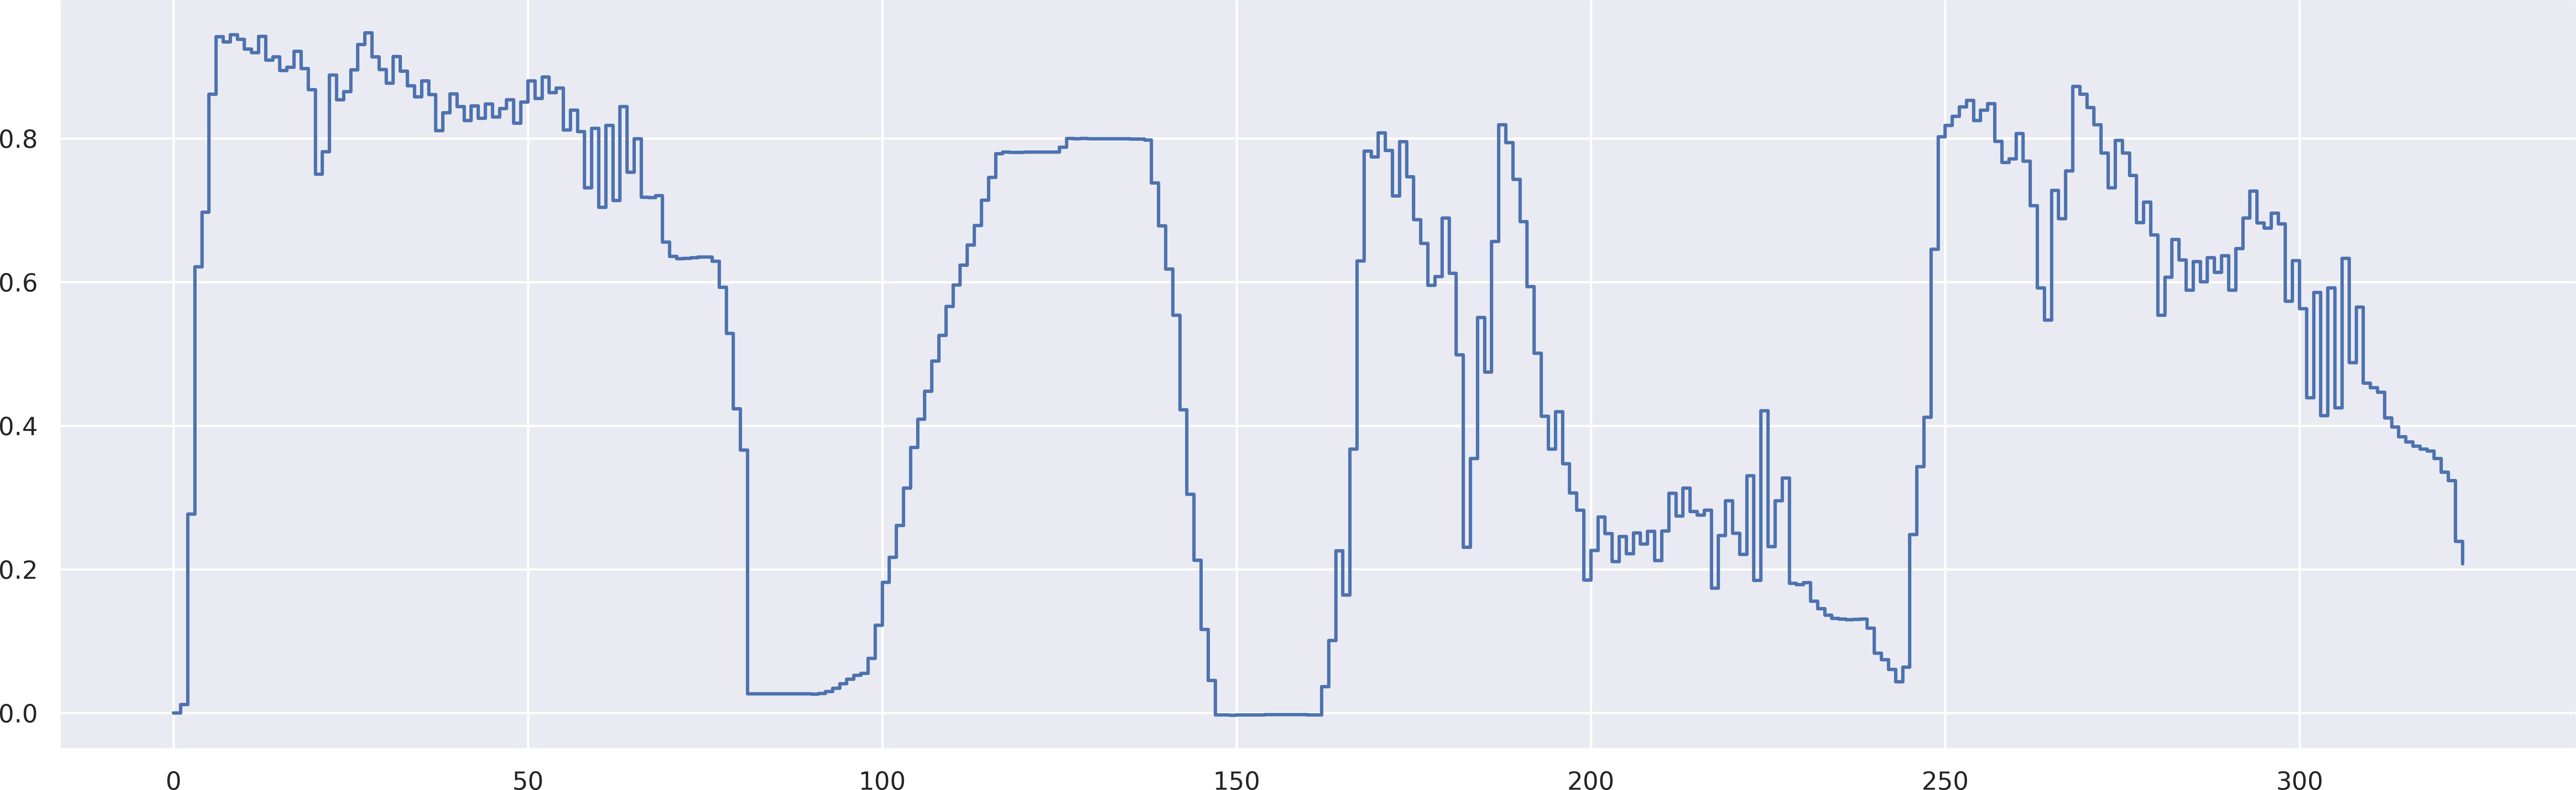
\includegraphics[width=\textwidth]{concat_mts_0815}
    \caption{\label{fig:concat_mts_0815} Concatenated, normalised, downsampled parameters NH, ALT, P30 and T30 from Flight 0815 for input to the mutlilayer perceptron.}
\end{figure}

The corresponding output consists of seven decimal damage values.

\subsection{Multivariate Time Series} \label{sec:prac:dataset:mts}
This dataset comprises the downsampled multivariate time series for all four parameters. The input for each flight was therefore an array with shape \(\left(4,\,81\right)\).

In the classification model, the output was a one-hot array containing 28 binary values in the given data or 28 probabilities in the predicted data (Section \ref{sec:data:classification_rep}). For the regression model, output data comprised seven decimal damage values.

\section{Model Types}
Three model architectures were implemented for this research; these will be described in the following.

In this section, the term `model' refers to the \textit{architecture} of the model implementation, which remains constant and is independent of the dataset used to train it. In the Results and Discussion (Section \ref{sec:discussion}), the term will be used to refer to an instance of \texttt{model} as generated by the code, which is influenced by the input data used to train it.

\subsection{Polynomial Regression} \label{sec:res:polyreg}
The first model implemented was a supervised machine learning method implemented with the \texttt{sklearn} library, based on the \ac{pr} method as described in Section \ref{sec:polyreg}.

The model was trained on two datasets: key values, and key values with features. It was repeated for polynomial degrees of 1 to 4, from which the highest scoring results were identified and documented (Sections \ref{sec:res:polyreg:kvs} and \ref{sec:res:polyreg:kvfs}).

The main code snippet from this model was as follows:

\begin{lstlisting}[language=Python]
for degree in range(1, 6):
    model = make_pipeline(
        StandardScaler(),
        PolynomialFeatures(degree),
        LinearRegression(),
        )

    model.fit(X_train, y_train)
    y_pred = model.predict(X_val)
\end{lstlisting}

Here, a data pipeline (using \texttt{make\_pipeline} from the \texttt{sklearn.pipeline} module) is constructed that consists of the \texttt{StandardScaler} for normalising the data, a transformation from a polynomial to a linear problem using \texttt{PolynomialFeatures}, followed by a linear regression of the data using the \texttt{LinearRegression} class. The model is fitted to the data and used to make a prediction \texttt{y\_pred}, from which the errors and scores are subsequently determined. These steps are repeated for polynomial degrees from 1 to 5.

The \ac{pr} model took 2.4 seconds to train on the complete key value dataset, and 14.9 seconds on the complete dataset containing key values and features.

\subsection{Multilayer Perceptron}
Using the \texttt{MLPRegressor} class from \texttt{sklearn}, an \ac{mlp} was constructed. In accordance with findings by \citet{cheng_polynomial_2019} that \ac{mlp}s are essentially \ac{pr} models, this was also repeated for a number of hidden layers between 1 and 4 with 100 nodes each. The model was trained until either convergence occurred, defined in this case as no improvement in loss by more than \num{1e-4} for ten epochs, or until the 500th epoch was reached.

The following code snippet is the main section of the \ac{mlp} model.

\begin{lstlisting}[language=Python]
for degree in range(1, 6):
    model = make_pipeline(
        StandardScaler(),
        MLPRegressor(hidden_layer_sizes=[100] * degree,
                     tol=1e-4, max_iter=500),
        )

    model.fit(X_train, y_train)
    y_pred = model.predict(X_val)
\end{lstlisting}

The \ac{mlp} model took 54.0 seconds to train on the complete key value dataset, 17.2 seconds on the complete dataset containing key values and features, and 91.9 seconds on the complete concatenated multivariate time series dataset.

\subsection{Convolutional Neural Network}
For the \ac{cnn} model, code was adapted from the repository\footnote{\url{https://github.com/hfawaz/InceptionTime}} created and published by \citet[]{fawaz_inceptiontime_2019}. Two types of task were attempted: time series classification and regression.

The code used to build the InceptionTime model is the following, which is an excerpt from one method of the \texttt{Classifier\_INCEPTION} class:

\begin{lstlisting}[language=Python]
def build_model(self, input_shape, nb_classes):
    input_layer = keras.layers.Input(input_shape)
    x = input_layer
    input_res = input_layer

    for d in range(self.depth):
        x = self._inception_module(x)

        if self.use_residual and d % 3 == 2:
            x = self._shortcut_layer(input_res, x)
            input_res = x

    gap_layer = keras.layers.GlobalAveragePooling1D()(x)
    output_layer = keras.layers.Dense(
        28, activation='softmax')(gap_layer)

    model = keras.models.Model(
        inputs=input_layer, outputs=output_layer)
\end{lstlisting}

The model comprises an input layer, a number (\texttt{depth}) of Inception modules based on the one described in Section \ref{sec:theory:inception}, a global average pooling layer, a fully connected layer and a final output layer. In the code snippet, the activation of the output layer is given as \texttt{'softmax'} with 28 output values as this model is used for classification; in the regression task, activation is simply changed to \texttt{'relu'} and the number of output values to 7.

If the \texttt{use\_residual} attribute of the class is set to \texttt{True}, residual connections (in the form of a \texttt{shortcut\_layer}) are included between every three layers of the model. The model used in this thesis employed residual connections.

The complete architecture is visualised in Figure \ref{fig:inceptiontime_archi}.

\begin{figure}[tb!]
    \centering
    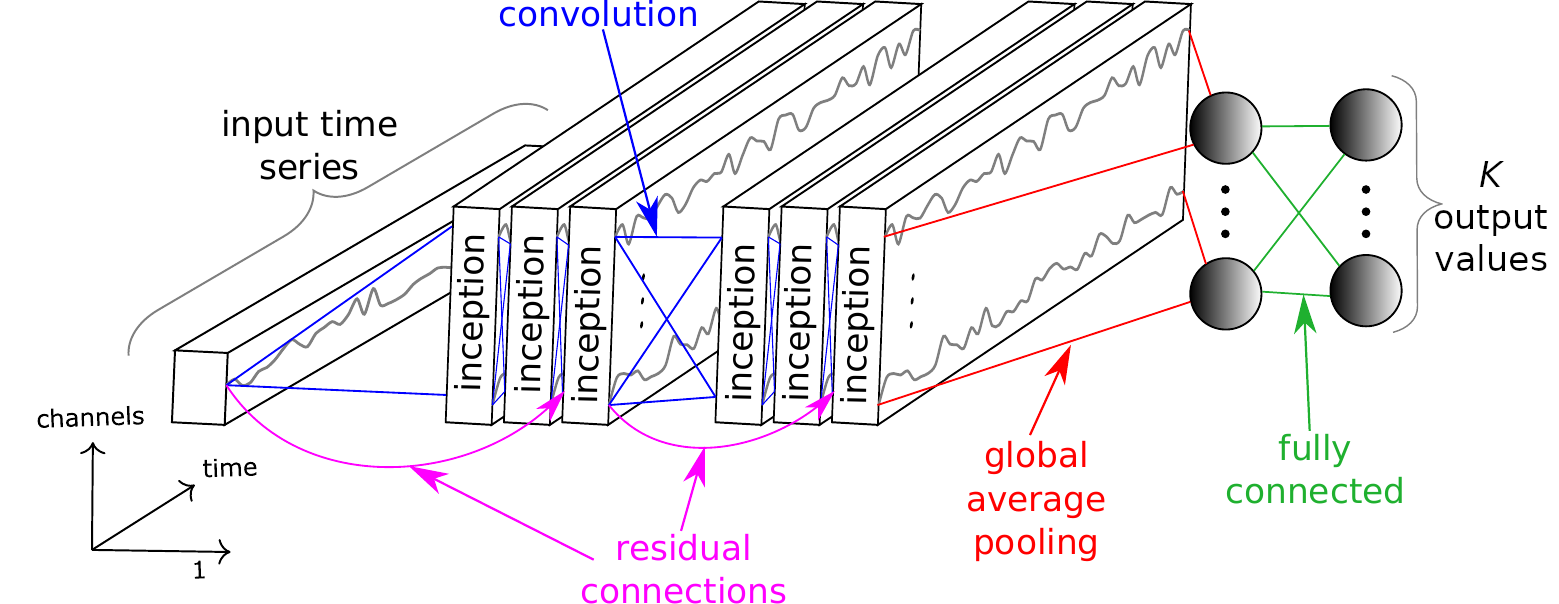
\includegraphics[width=\textwidth]{inceptiontime_archi}
    \caption{\label{fig:inceptiontime_archi} The architecture of the InceptionTime deep convolutional neural network, based on \citet{fawaz_inceptiontime_2019}.}
\end{figure}

The model was trained for both the classification and the regression task on the multivariate time series dataset.
